\chapter{Application of transmission line(2)}
We are discussing applications of transmission line, which are:
\begin{enumerate}[(i)]
\item Impedance measurement
\item As a circuit element
\item As a step up transformer
\item Impedance matching 
\end{enumerate}

In this chapter, we are considering:
\begin{enumerate}[(i)]
\item As a circuit element
\item As a step up transformer
\end{enumerate}

\section{As A Circuit Element}
At high frequency, inductor does not behave only as an inductor, but as a capacitor and an inductor. Also, a capacitor does not behave only as a capacitor, but as an inductor and a capacitor. Due to this behavior experienced by this lumped elements (capacitor and inductor) at high frequency, a \textbf{transmission line} is used as an inductor and as a capacitor.
At short circuit length $l_{sc}$ and\ open\ circuit\ length\ $l_{oc}$\ ,\ it\ is\ used \ as\ a\ capacitor\ and \ as \ an\ inductor\ by\ varying\ its\ length.\\
Recall from chapter 10,\\
For an inductor: $0 \textless l_{sc} \textless 
\frac{\lambda}{\small 4}$\\
For\ a\ capacitor: $\frac{\lambda}{4} \textless l_{sc} \textless \frac{\lambda}{2} $


Up to this point, we have dealt with lossless transmission line, which imply, for the use of open or short circuit transmission line as a circuit element, we expect to get an infinite quality factor especially in a case were we used it as a resonance circuit at a particular length. \textbf{Quality factor} of a resonance circuit depends on the losses of the circuit, higher loss leads to low quality factor and vice versa.

Now, we consider a transmission line with losses at length of $ l=\frac{\lambda}{4} $, so\ that we can then determine the actual value of quality factor for this case.\\

Let the length be $ l=\frac{\lambda}{4} $, either open circuit or short circuit as shown in figure 11.1.
\begin{figure}[h]
\centering
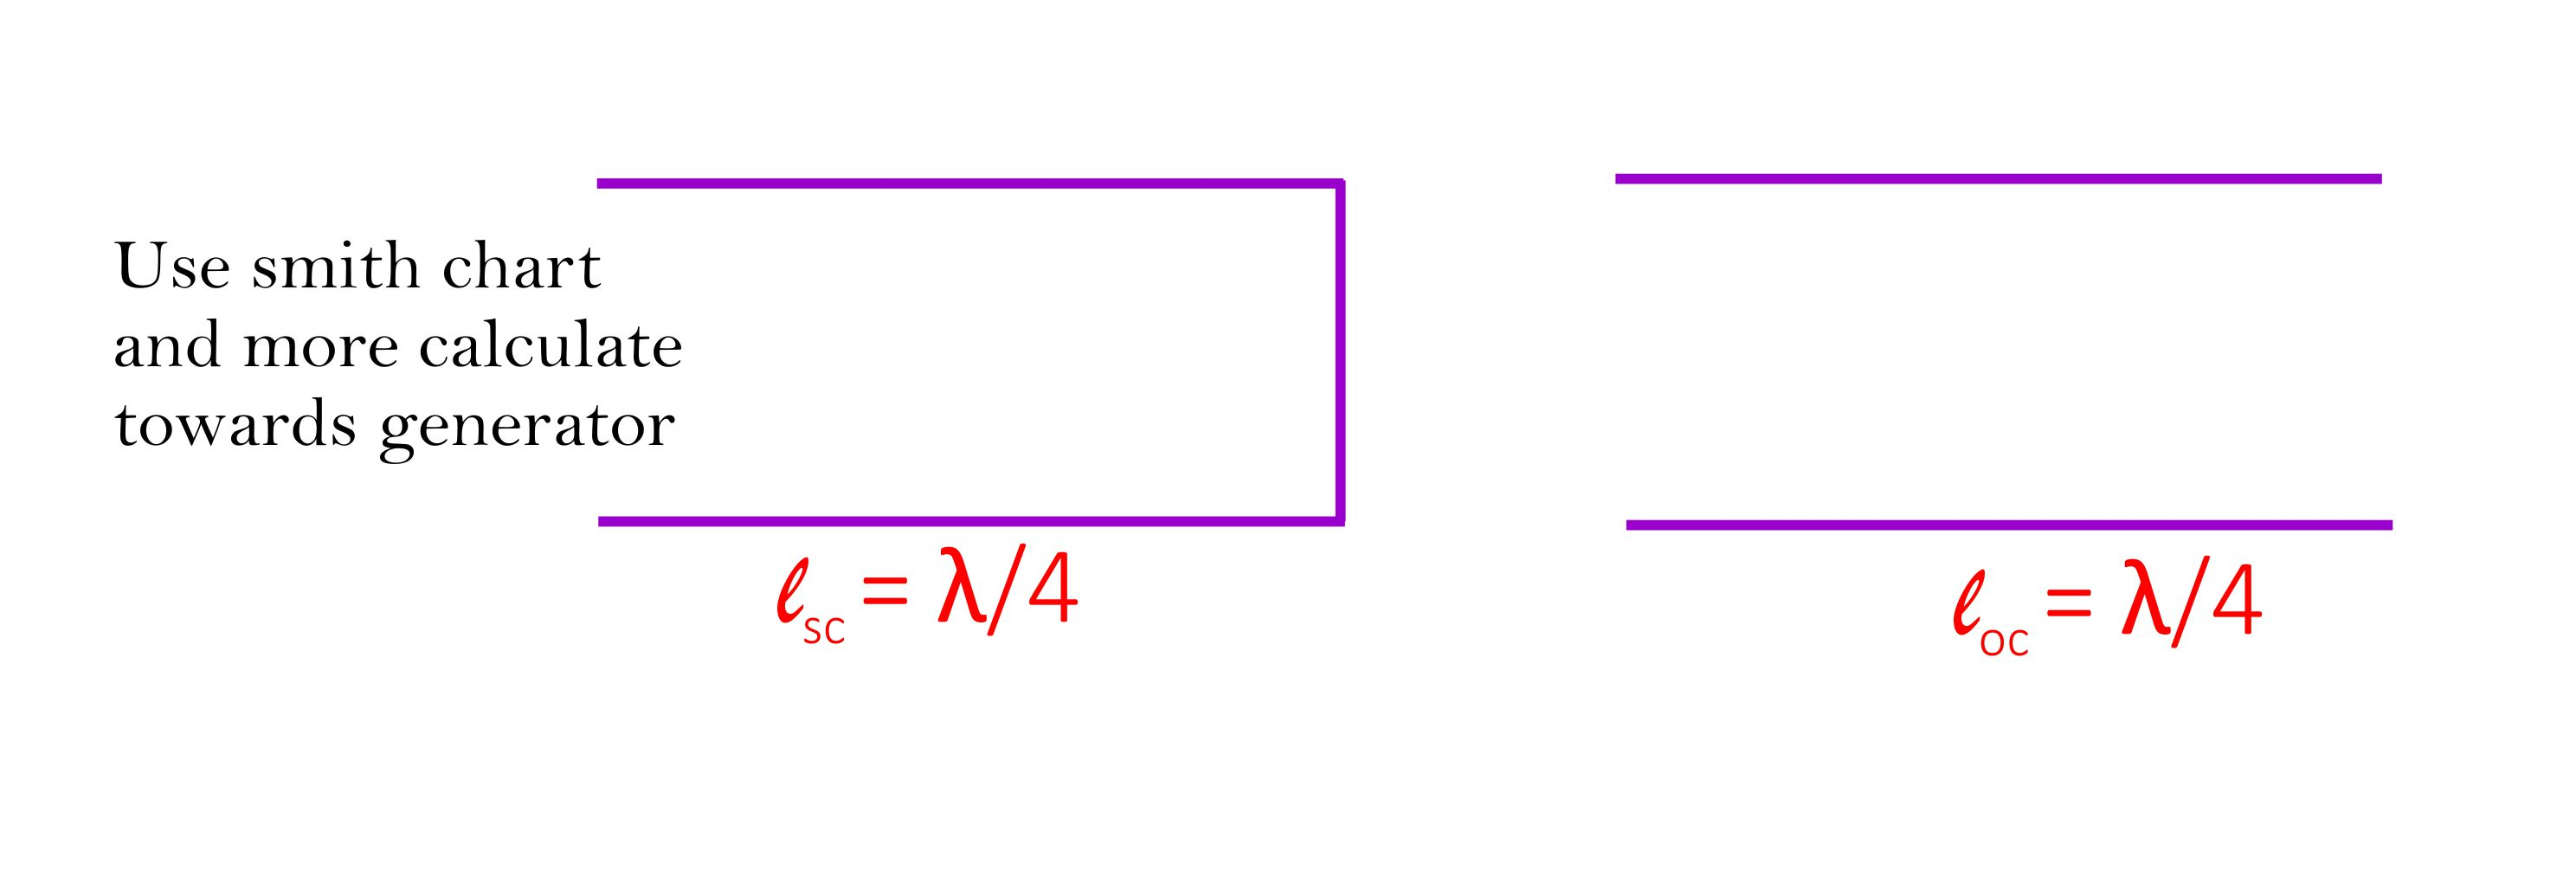
\includegraphics[width=1\linewidth]{./graphics/fig1}
\caption{Diagram of a short circuit and open circuit transmission line of length $\frac{\lambda}{4}$}
\end{figure}
At $ \frac{\lambda}{4} $, the open circuit will appear as a short circuit to the line and the short circuit will appear as an open circuit.\\

At $ \footnote{Short circuit length}l_{sc}=\frac{\lambda}{4} $, it will appear as a parallel resonance circuit and $ \footnote{Open circuit length}l_{oc}=\frac{\lambda}{4} $, it will appear as a series resonance circuit.\\
So, we calculate the actual input impedance of these lines with losses and then go on to calculate the quality factor.\\
To calculate the input impedances: $ Z_{oc} $ and $ Z_{sc} $, for a length $ l=\frac{\lambda}{4} $ with losses.\\
Recall impedance transformation relationship
\begin{equation}
\footnote{Impedance at any point on the line}Z(l) = Z_{o}\left(\frac{Z_{L}\cosh\gamma l + Z_{o}\sinh\gamma l}{Z_{o}\cosh\gamma l + Z_{L}\sinh\gamma l}\right)
\end{equation}
At short circuit length, $ \footnote{Impedance at load point}Z_{L}=0 $
\begin{equation}
Z(l)_{sc} = Z_{o}\left( \frac{0\cosh\gamma l + Z_{o}\sinh\gamma l}{Z_{o}\cosh\gamma l + 0\sinh\gamma l}\right) 
\end{equation} 
\begin{equation}
Z(l)_{sc} = Z_{o}\left(\frac{Z_{o}\sinh\gamma l}{Z_{o}\cosh\gamma l}\right)
\end{equation}
\begin{equation}
Z(l)_{sc} = Z_{o}\left(\frac{\sinh\gamma l}{\cosh\gamma l}\right)
\end{equation}

From trigonometry function:
$ \tanh\theta =\frac{\sinh\theta}{\cosh\theta} $
\begin{equation}
\boxed{Z(l)_{sc}=Z_{o}\tanh\gamma l}	\end{equation}

We adjust the expression for open circuit length at $ Z_{L} =\infty $ \\
Recall impedance transformation relationship
\begin{equation}
Z(l) = Z_{o}\left(\frac{Z_{L}\cosh\gamma l + Z_{o}\sinh\gamma l}{Z_{o}\cosh\gamma l + Z_{L}\sinh\gamma l}\right)
\end{equation}
Dividing the numerator and denominator by $ Z_{L} $
\begin{equation}
Z(l)_{oc} = Z_{o}\left(\frac{\cosh\gamma l +\frac{Z_{o}}{Z_{L}}\sinh\gamma l}{\frac{Z_{o}}{Z_{L}}\cosh\gamma l+ \sinh\gamma l}\right)
\end{equation}
At $ Z_{L}=\infty $ \\
$ \frac{Z_{o}}{Z_{L}} =\frac{Z_{o}}{\infty} = 0 $ 
\begin{equation}
Z(l)_{oc} = Z_{o}\left(\frac{\cosh\gamma l}{\sinh\gamma l}\right)
\end{equation} 
From trigonometry:\\
$ \frac{1}{\tanh\theta}=\frac{\cosh\theta}{\sinh\theta}=\coth\theta $
\begin{equation}
\boxed{Z(l)_{oc}=Z_{o}\coth\gamma l}	
\end{equation}

$ Z(l)_{sc}=Z_{o}\tanh\gamma l $ and $ Z(l)_{oc}=Z_{o}\coth\gamma l $, but with $ \gamma=\alpha +j\beta $, we have $ \alpha<<\beta $ for low loss line (not lossless in this case), i.e $ \gamma\neq j\beta $ only, the $ \alpha $ part must be taken into consideration also. We know that at $ l=\frac{\lambda}{4} $, the input impedance of a short circuit line is an open circuit and that of an open circuit line is a short circuit. However, in the presence of a loss, that will not be true. The impedance will neither be infinity for $ Z_{sc} $ and zero for $ Z_{oc} $. If the loss is present, the input impedance will give:\\
\begin{equation}
Z_{sc}=Z_{o}\tanh\gamma l=Z_{o}\tanh(\alpha+j\beta)l
\end{equation}
where $ \gamma=\alpha+j\beta $ (In the case of lossy transmission line).\\

From trigonometry:
$\tanh(A+B)=\frac{\tanh A+\tanh B}{1+\tanh A\tanh B} $

\begin{equation}
\tanh(\alpha+j\beta)l=\frac{\tanh (\alpha l) + \tanh (j\beta l)}{1 + \tanh (\alpha l)\tanh (j\beta l)}
\end{equation}

Recall that: $ \tanh jA= j\tan A $\\
Therefore,
\begin{equation}
Z_{o}\tanh(\alpha+j\beta)l=Z_{o}\left(\frac{\tanh \alpha l+j\tan \beta l}{1+j\tanh \alpha l\tan \beta l}\right)
\end{equation}
If $ \alpha $ is small compare to $ \beta $ for a length of $ \frac{\lambda}{4} $ of transmission line, $ \alpha l $ is much smaller than 1. For a low loss line, $ \alpha<<\beta $ and $ \beta=\frac{2\pi}{\lambda} $. Therefore	$ \tanh \alpha l \simeq \alpha l $, then we have
\begin{equation}
Z_{sc}\simeq Z_{o}\left(\frac{\alpha l + j \tan \beta l}{1+ j\alpha l \tan\beta l}\right)
\end{equation} 
For $ l=\frac{\lambda}{4} $, $ \beta=\frac{2\pi}{\lambda} $\\
$ \beta l= \frac{2\pi}{\lambda} \times\frac{\lambda}{4} =\frac{\pi}{2} $\\
Dividing both the numerator and denominator by $ \tan\beta l $
\begin{equation}
Z_{sc}=Z_{o}\left(\frac{\alpha l + j \tan \beta l}{1+ j\alpha l \tan\beta l}\right)\times\left(\frac{\frac{1}{\tan \beta l}}{\frac{1}{\tan \beta l}}\right)
\end{equation}
\begin{equation}
Z_{sc}=Z_{o}\left(\frac{\frac{\alpha l}{\tan \beta l}+\frac{j\tan \beta l}{\tan \beta l}}{\frac{1}{\tan \beta l}+\frac{j\alpha l\tan \beta l}{\tan \beta l}}\right)
\end{equation}
\begin{equation}
Z_{sc}=Z_{o}\left(\frac{\frac{\alpha l}{\tan \beta l} + j}{\frac{1}{\tan \beta l} + j\alpha l}\right)
\end{equation}
$ \tan \beta l =\tan\frac{\pi}{2}=\infty $
\begin{equation}
Z_{sc}=Z_{o}\left(\frac{\frac{\alpha l}{\infty} + j}{\frac{1}{\infty} + j \alpha l}\right)
\end{equation}\\
$ \frac{\alpha l}{\infty}=0, \frac{1}{\infty}=0  $
\begin{equation}
Z_{sc}=Z_{o}\left(\frac{j}{j\alpha l}\right)=Z_{o}\left(\frac{1}{\alpha l}\right)
\end{equation}
\begin{equation}
\boxed{Z_{sc}=\frac{Z_{o}}{\alpha l}}	\end{equation}

Therefore, this means that the input impedance of a short circuit line, if the length is $ \frac{\lambda}{4} $ is $ \frac{Z_{o}}{\alpha l} $, which is not infinity. Recall:$ Z_{sc} $ = $ \infty $ for lossless line scenario, but $ \alpha l << 1 $ means $ Z_{sc} $ is large but not infinity.\\

Similarly,\\
 $ Z_{oc}=Z_{o}\coth\gamma l=\frac{Z_{o}}{\tanh\gamma l} $\\\\
$ Z_{oc}=Z_{o}\coth\gamma l=Z_{o}\coth(\alpha+j\beta) l $\\\\
For low loss transmission line $ \alpha<<\beta $ \\\\Recall,\\
$ \tanh(\alpha+j\beta)l=\frac{\tanh (\alpha l) + \tanh (j\beta l)}{1 +j \tanh (\alpha l)\tanh (j\beta l)} $\\\\
$ \frac{1}{\tanh(\alpha+j\beta)l}=\frac{1 + j\tanh (\alpha l)\tanh (j\beta l)}{\tanh (\alpha l) + \tanh (j\beta l)} $\\\\
$ \tanh jA= j \tan A $\\\\
$ \tanh(\alpha+j\beta)l=\frac{\tanh \alpha l+j\tan \beta l}{1+j\tanh \alpha l\tan \beta l} $\\\\
$ \frac{1}{\tanh(\alpha+j\beta)l}=\frac{1+j\tanh \alpha l\tan \beta l}{\tanh \alpha l+j\tan \beta l} $

\begin{equation}
Z_{oc} = \frac{Z_{o}}{\tanh(\alpha+j\beta)}=Z_{o}\left(\frac{1+j\tanh \alpha l\tan \beta l}{\tanh \alpha l+j\tan \beta l}\right)
\end{equation}
\begin{equation}
Z_{oc} \simeq Z_{o}\left(\frac{1+ j \alpha l\tan \beta l}{\alpha l+j\tan \beta l}\right)
\end{equation}\\\\
Divide both the numerator and denominator by $ \tan \beta l $
\begin{equation}
Z_{oc}=Z_{o}\left(\frac{\frac{1}{\tan \beta l}+\frac{j \alpha l\tan \beta l}{\tan \beta l}}{\frac{\alpha l}{\tan \beta l}+\frac{j\tan \beta l}{\tan \beta l}}\right)
\end{equation}
\begin{equation}
=Z_{o}\left(\frac{\frac{1}{\tan \beta l} + j \alpha l}{\frac{\alpha l}{\tan \beta l} + j}\right)
\end{equation}\\
Recall,\\
$ \tan\beta l =\tan\frac{\pi}{2}=\infty $\\
\begin{equation}
Z_{oc}=Z_{o}\left(\frac{\frac{1}{\infty} + j \alpha l}{\frac{\alpha l}{\infty} + j}\right)
\end{equation}
$ \frac{1}{\infty}=0, \frac{\alpha l}{\infty}=0 $\\
\begin{equation}
\boxed{	Z_{oc}=Z_{o}\left(\frac{j \alpha l}{j}\right)=Z_{o}(\alpha l)}\end{equation}\\
Therefore, for low loss condition:\\
 $ Z_{sc}\simeq \frac{Z_{o}}{\alpha l} $\\
$ Z_{oc} \simeq Z_{o} \alpha l $\\ 

Ideally $ Z_{oc}=0 $, but this is not the case with low loss line where we have  $ Z_{oc} = Z_{o} \alpha l $. What we note here is that, the input impedance of the resonance section of a transmission line is ideally zero or infinity for series or parallel resonance circuit. In practice, we see that we have small input impedance for a series resonance circuit and large input impedance for parallel resonance circuit.\\

With $ Z_{oc} =  Z_{o} \alpha l $ and  
$ Z_{sc}= \frac{Z_{o}}{\alpha l} $, we can vary the frequency and measure the variation of $ Z_{sc} $ or $ Z_{oc} $ with frequency. Recall that $ \alpha $ depends on frequency; length $(l)$ depends on frequency too since  $ l=\frac{\lambda}{4} $. The variation of $ Z_{sc} $  or  $ Z_{oc} $ with frequency gives us what is called the \textbf{frequency response of the circuit}.\\

Quality factor can be calculated in two ways:\\
1. From the frequency response of the circuit\\
2. From the basic definition of quality factor.\\

By definition,
\begin{dmath}
Quality factor(Q) =2\pi\left(\frac{ energy\ stored\ in\ the\ circuit  }{Energy\ lost\ per\ cycle}\right) 
\end{dmath}  
If the resonant frequency is $ f_{o} $, the energy lost per cycle is $ f_{o} $ cycles per seconds. Since in 1 seconds, we have $ f_{o} $ number of cycles;\\
\begin{dmath}
Quality factor Q=2 \pi f_{o}\left(\frac{energy\ stored\ in\ the\ circuit }{Energy\ lost\ per\ second}\right)
\end{dmath}
 Energy lost per second = Power loss in the circuit  
\begin{dmath}
Quality factor (Q)=2 \pi f_{o}\left(\frac{energy\ stored\ in\ the\ circuit }{Power\ loss\ in\ the\ circuit}\right)
\end{dmath}

So to calculate the quality factor, we calculate the energy stored in a section of the transmission line and the power loss in the transmission line. Then we can easily find out the value for the quality factor for that section of transmission line.\\

Alternatively, the quality factor is related to the frequency response. If we plot the current or voltage response when a current or voltage source is applied to the input section of the transmission line and measure the 3dB bandwidth of the response, the center frequency divided by the 3dB bandwidth of the frequency response gives the \textbf{quality factor}. 
\begin{figure}[h]
\centering
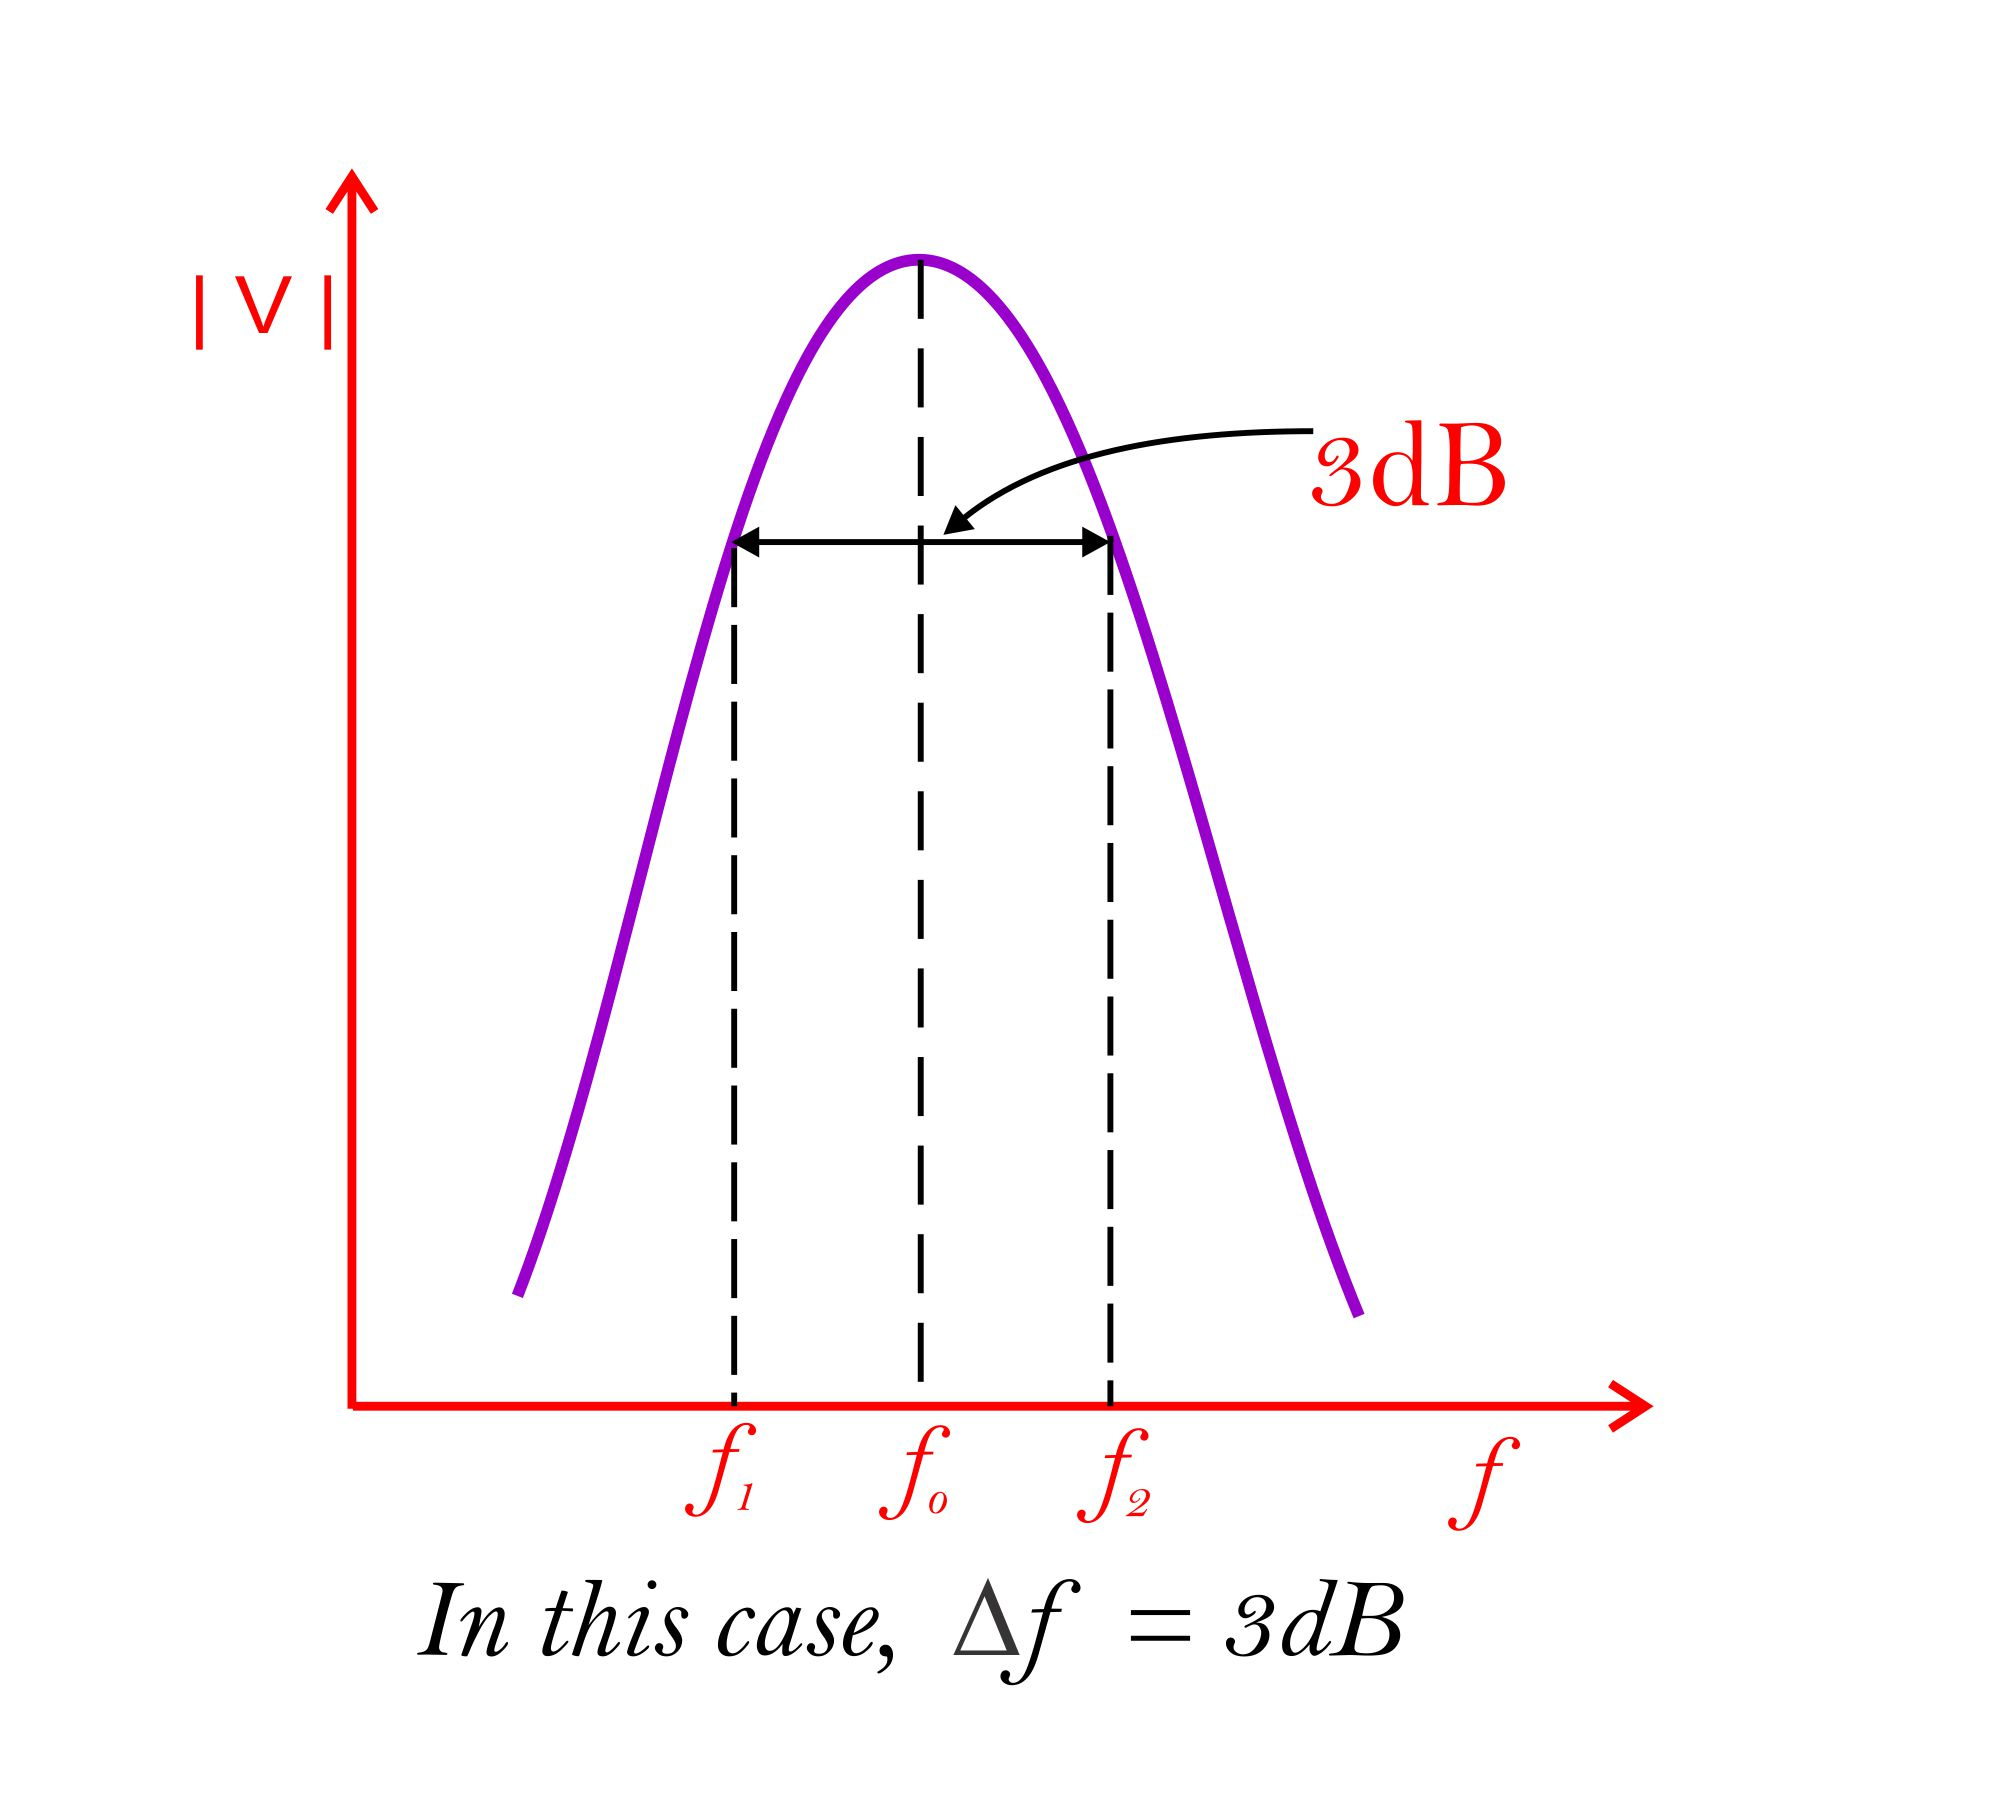
\includegraphics[scale=0.6]{./graphics/fig2}
\caption{Graph showing the voltage response}
\end{figure}It doesn't matter if we use a series or parallel resonance circuit. The voltage response is shown in figure 11.2. At resonance frequency $ f_{o} $, we get the maximum response below and beyond that frequency in which the amplitude drops. The 3dB frequency is where the amplitude reduces to $ \frac{1}{\sqrt{2}} $ of its maximum value of the response. In this case,\\ $ \Delta f=3dB $ bandwidth,\\ $ \Delta f=f_{2}-f_{1} $,\\
\begin{equation}
\boxed{	Q=\frac{f_{o}}{\Delta f}=\frac{f_{o}}{f_{2}-f_{1}}}\end{equation}\\
Hence, the quality factor can be calculated from the impedance calculation as this will give the frequency response.\\
Alternatively, take a section of transmission line, find the voltage distribution and current distribution in the transmission line, then calculate the power loss. Use this information to calculate the quality factor.\\
Recall,
\begin{equation}
Q=2\pi f_{o}\left(\frac{Energy\ stored\ in\ circuit}{Power\ loss\ in\ circuit}\right)
\end{equation}
Using this method to calculate quality factor(Q),
lets consider a section of transmission line of $ l=\frac{\lambda}{4} $ and say the line is short circuited for this specific case.\\
The length cannot be constant at all frequencies since $ l=\frac{\lambda}{4} $, so lets say frequency = $ f_{o} $ when $ l=\frac{\lambda_{o}}{4} $. 

Hence, the resonant frequency of a circuit is $ f_{o} =\frac{V}{\lambda_{o}}$ (where v = velocity of the wave). We can get voltage and current expression on the transmission line with the load short circuited. With load short circuited $(Z_{L}=0) $, the reflection coefficient at the load point is -1 as we have seen earlier. So $ \Gamma_{L} = \frac{Z_{L} - Z_{o}}{Z_{L} + Z_{o}} = \frac{0 - Z_{o}}{0 + Z_{o}} = -1 $. This is saying that the amplitude of reflection coefficient is 1 with a phase change of $ 180^{o} $. We will make use of this information later when we talk about the  application of transmission line for voltage and current stepping up transformers.

At this point, we can write down the voltage and current equation since we know the reflection coefficient. We can also find out what the variation of voltage and current is on the transmission line.
\begin{equation}
\footnote{voltage along any length on the trasmission line}V(l) = V^{+}e^{j\beta l} + V^{-}e^{-j\beta l} 
\end{equation}
Because : $ \frac{V^{-}}{V^{+}} = \Gamma, V^{-} = -V^{+}$
\begin{equation}
V(l) = V^{+}e^{j\beta l} - V^{+}e^{-j\beta l}
\end{equation}
Recall from Euler formula:
\begin{equation*}
\frac{e^{j\beta l }- e^{-j\beta l}}{2j} = \sin \beta l
\end{equation*}
\begin{equation}
j2V^{+}\left(\frac{e^{j\beta l }- e^{-j\beta l}}{2j}\right) =j2V^{+}\sin \beta l
\end{equation}
Let: $ j2V^{+} = V_{o}$
\begin{equation}
j2V^{+}\sin \beta l = V_{o}\sin \beta l 
\end{equation}
\begin{equation}
\boxed{ | V(l) | = |V_{o}\sin \beta l |} \end{equation}
In a similar manner for current:
\begin{equation}
\footnote{current at any length on the transmission line}I(l) = \frac{V^{+}}{Z_{o}}e^{j\beta l} - \frac{V^{-}}{Z_{o}}e^{-j\beta l} 
\end{equation}
Because : $ \frac{V^{-}}{V^{+}} = \Gamma, V^{-} = -V^{+}$
\begin{equation}
I(l) = \frac{V^{+}}{Z_{o}}e^{j\beta l} + \frac{V^{+}}{Z_{o}}e^{-j\beta l} 
\end{equation}
recall:
\begin{equation*}
\frac{e^{j\beta l} + e^{-j\beta l}}{2} = \cos \beta l
\end{equation*}
\begin{equation}
\frac{2V^{+}}{Z_{o}}(\frac{e^{j\beta l} + e^{-j\beta l}}{2}) =\frac{2V^{+}}{Z_{o}}\cos \beta l
\end{equation}
Let: $ 2V^{+} = V_{o}$
\begin{equation}
\boxed{| I(l) | = \left|\frac{V_{o}}{Z_{o}}\cos \beta l \right|}\end{equation}\\
So plotting this voltage and current along a short circuit transmission line, we have the variation shown in figure 11.3 . \\
At $ l = \frac{\lambda}{4}$ , $ \beta l = \frac{\pi}{2} $. So that $\sin \beta l = \sin \frac{\pi}{2}$ = 1, $\cos \beta l = \cos \frac{\pi}{2} = 0$. 

For the voltage distribution we have a peak at $ l = \frac{\lambda}{4}$ and a minimum of $ l = 0$.\\ For current variation we have a peak value at  $ l = 0$ and a minimum value at $l = \frac{\lambda}{4}$ as shown on the graph of voltage and current distribution on the transmission line.
\begin{figure}[h]
\centering
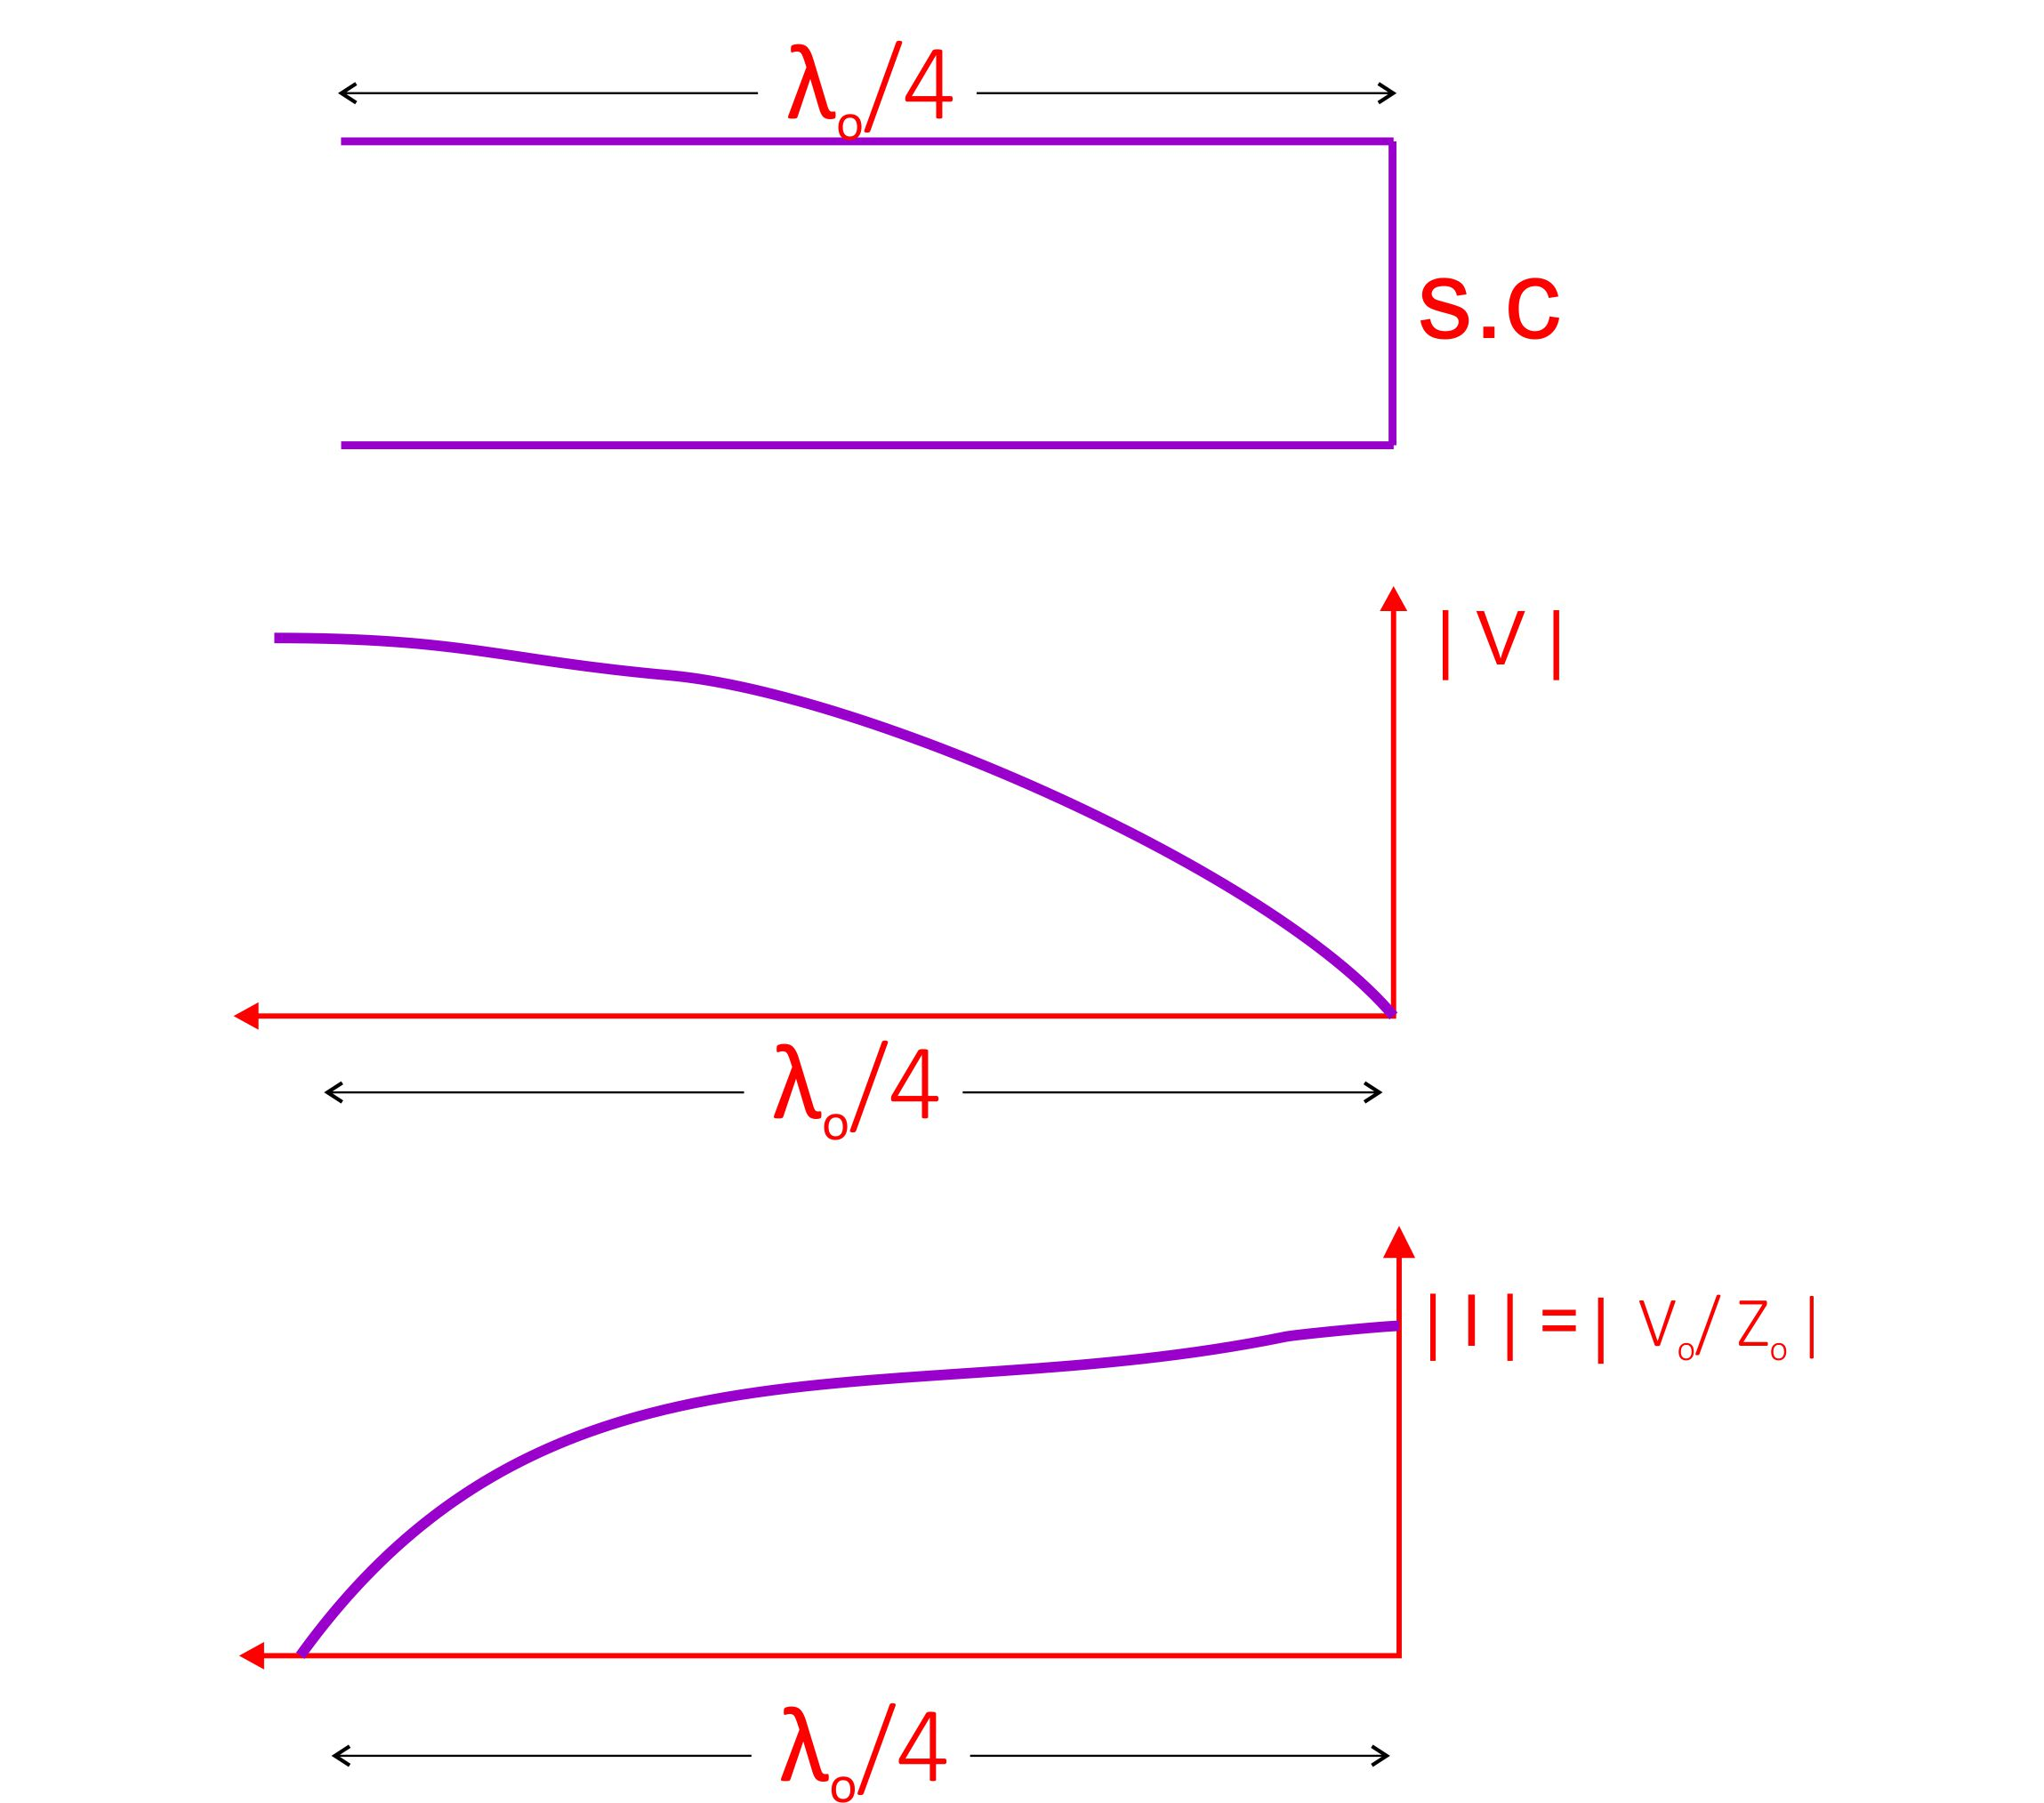
\includegraphics[width=1\linewidth]{./graphics/fig03}
\caption{voltage and current wave of a short circuit transmission line }
\end{figure}

Now we know the voltage and current variation on a section of this transmission line. Hence, we can find the energy stored at different section of the transmission line. To find the energy stored, the capacitance of a small section of a transmission line is $C\Delta l$ for $\Delta l$ section;since R, G, C and L are always stated per unit length. Hence, the capacitive energy stored in that section = $\frac{1}{2}$ C$\Delta $$l$ $ V^{2}$. The inductive energy in that section =  $\frac{1}{2}$ L$\Delta $$l$ $ I^{2}$. The total energy stored in a transmission line can be written as:
\begin{equation}
U = \frac{1}{2}C\int_{0}^{\frac{\lambda_{o}}{4}}|V(l)|^{2}dl + \frac{1}{2}L\int_{0}^{\frac{\lambda_{o}}{4}}|I(l)|^{2}dl
\end{equation}
From: $ | V(l) | = |V_{o}\sin \beta l | $ and $  | I(l) | = \left|\frac{V_{o}}{Z_{o}}\cos \beta l\right |$
\begin{equation}
U = \frac{1}{2}C\int_{0}^{\frac{\lambda_{o}}{4}}|V_{o}\sin \beta l |^{2}dl + \frac{1}{2}L\int_{0}^{\frac{\lambda_{o}}{4}}\left|\frac{V_{o}}{Z_{o}}\cos \beta l \right|^{2}dl
\end{equation}
\begin{equation}
U = \frac{1}{2}CV_{o}^{2}\int_{0}^{\frac{\lambda_{o}}{4}}(\sin^{2} \beta l) dl + \frac{1}{2}L\frac{V_{o}^{2}}{Z_{o}^{2}}\int_{0}^{\frac{\lambda_{o}}{4}}( \cos^{2} \beta l) dl    
\end{equation}
Recall from trigonometry:\\       
$\sin^{2} \beta l = \frac{1 - \cos2\beta l}{2}$, $\cos^{2} \beta l = \frac{1 + \cos2\beta l}{2}$
{\small \begin{equation}
 U = \frac{1}{2}CV_{o}^{2}\int_{0}^{\frac{\lambda_{o}}{4}}\left(\frac{1}{2} - \frac{\cos 2\beta l}{2}\right) dl + \frac{1}{2}L\frac{V_{o}^{2}}{Z_{o}^{2}}\int_{0}^{\frac{\lambda_{o}}{4}} \left
(\frac{1}{2} + \frac{\cos 2\beta l}{2}\right) dl    
\end{equation}}
\begin{equation}
= \frac{1}{2}CV_{o}^{2}\left[\frac{l}{2} - \frac{\sin 2\beta l}{4 \beta}\right]_{0}^{\frac{\lambda_{o}}{4}}  + \frac{1}{2}L\frac{V_{o}^{2}}{Z_{o}^{2}}\left[\frac{l}{2} + \frac{\sin 2\beta l}{4 \beta}\right]_{0}^{\frac{\lambda_{o}}{4}}
\end{equation}
{\smal
l\begin{equation}
= \frac{1}{2}CV_{o}^{2}\left[\frac{\lambda_{o}}{8} - \sin \frac{2(\frac{2\pi}{\lambda_{o}})\frac{\lambda_{o}}{4} }{4 \beta}\right] + \frac{1}{2}L\frac{V_{o}^{2}}{Z_{o}^{2}}\left[\frac{\lambda_{o}}{8} + \frac{\sin 2(\frac{2\pi}{\lambda_{o}})\frac{\lambda_{o}}{4} }{4 \beta}\right]
\end{equation}}
\begin{equation}
= \frac{1}{2}CV_{o}^{2}\left[\frac{\lambda_{o}}{8} -  \frac{\sin \pi}{4 \beta}\right] + \frac{1}{2}L\frac{V_{o}^{2}}{Z_{o}^{2}}\left[\frac{\lambda_{o}}{8} + \frac{\sin \pi}{4 \beta}\right]
\end{equation}
\begin{equation}
= \frac{1}{2}CV_{o}^{2}\left[\frac{\lambda_{o}}{8}\right] + \frac{1}{2}L\frac{V_{o}^{2}}{Z_{o}^{2}}\left[ \frac{\lambda_{o}}{8} \right]
\end{equation}
Where: $\frac{1}{2}CV_{o}^{2}\left[\frac{\lambda_{o}}{8}\right] $ = energy stored in line capacitance;\\
and  $ \frac{1}{2}L\frac{V_{o}^{2}}{Z_{o}^{2}}\left[ \frac{\lambda_{o}}{8} \right] $ = energy stored in line inductance.\\
We see that the two quantities are equal since:
\begin{equation*}
Z_{o} = \sqrt{\frac{L}{C}}
\end{equation*}
\begin{equation*}
CZ_{o}^{2} = L,
 C= {\frac{L}{Z_{o}^{2}}}
\end{equation*}
  
\begin{equation}
U= \frac{1}{2}CV_{o}^{2}\left[\frac{\lambda_{o}}{8}\right] +\frac{1}{2}CV_{o}^{2}\left[\frac{\lambda_{o}}{8}\right]
\end{equation}
Therefore, the total energy stored is:
\begin{equation}
U= \frac{1}{2}CV_{o}^{2}\left[\frac{\lambda_{o}}{4}\right] 
\end{equation}

To calculate the quality factor, we also need to calculate the power loss in the transmission line. Hence, we go back to the primary parameters of the transmission line R, L, G and C. If we take the section of a transmission line $\frac{\lambda_{o}}{4}$ shown in figure 11.4.
\begin{figure}[h]
\centering
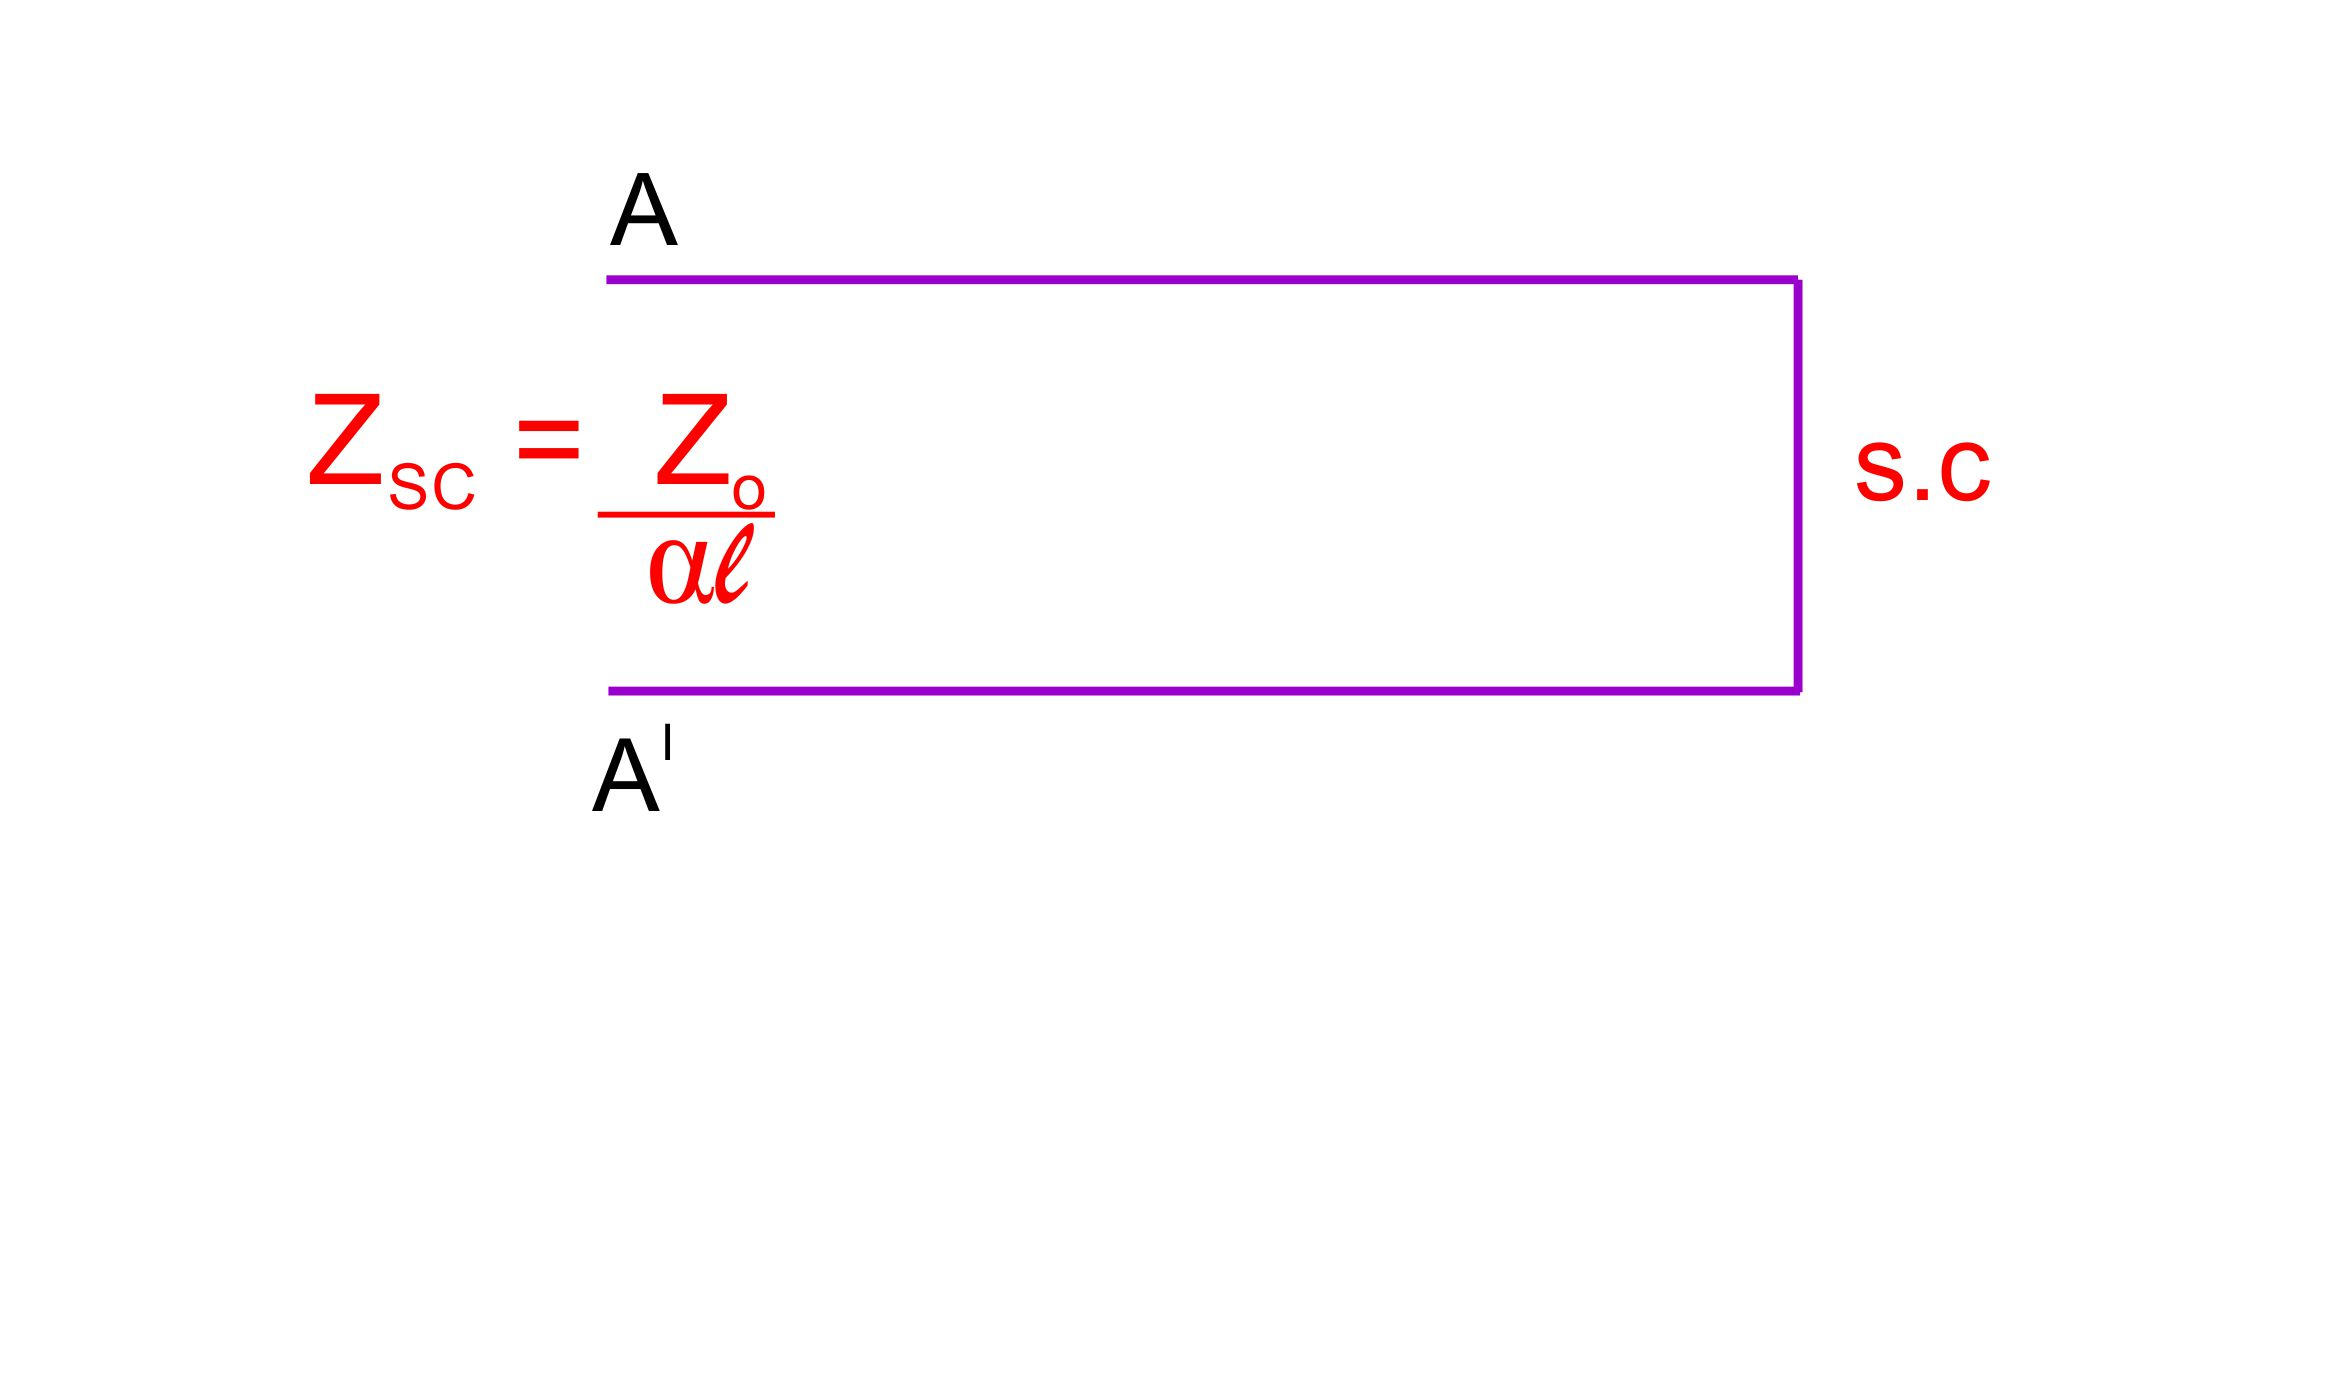
\includegraphics[width=1\linewidth]{./graphics/fig4}
\caption{Diagram showing the input impedance of a short circuit transmission line}
\end{figure}

The energy stored in the line is connected at point AA'. Finding out what the power loss at AA' is, the power loss is equivalent to the power loss in the line because the line is short circuited. Therefore, the load is not consuming any power and the power supplied will be equal to the loss in the transmission line. So without going into the primary constant of the transmission  line, just by calculating the input impedance of the line, we can find out what the equivalent resistance would be at the input point of the line and find out the losses through this resistance;that will be the power loss in the line. Hence, the input impedance seen at AA' will be
\begin{equation}
Z_{sc} = \frac{Z_{o}}{\alpha l}
\end{equation}
and power loss:
\begin{equation}
P_{loss} = \frac{V_{o}^{2}}{Z_{sc}} = \frac{V_{o}^{2}}{\frac{Z_{o}}{\alpha l}}
\end{equation}
$ V_{o} $ is the supplied voltage:
\begin{equation}
V_{o} = \frac{V_{o}^{2}}{Z_{o}}*\alpha *\frac{\lambda_{o}}{4}
\end{equation}
Recall,
  
Q = $ 2 \pi f_{o} \left(\frac{\ energy\ stored\ in\ a\ circuit}{power\ loss\ in\ the\ circuit}\right)$
\begin{equation}
Q = 2 \pi f_{o}\left(\frac{\frac{1}{2}*CV_{o}^{2}*\frac{\lambda_{o}}{4}}{ \frac{V_{o}^{2}}{Z_{o}}*\alpha *\frac{\lambda_{o}}{4}}\right)
end{equation}
\begin{equation}
Q = 2 \pi f_{o}\left(\frac{\frac{1}{2}C}{\frac{\alpha}{Z_{o}}}\right)
\end{equation}
\begin{equation}
Quality\ factor (Q) = \frac{2 \pi f_{o} Z_{o}C}{2\alpha}
\end{equation}
But $ Z_{o} = \sqrt{\frac{L}{C}}$\\
$ Z_{o}*C = \sqrt{\frac{L}{C}} * C =\sqrt{\frac{L}{C}} * \sqrt{C^{2}} = \sqrt{LC}$\\
$ 2\pi f_{o} = \omega_{o} $\\
But $ \footnote{Angular velocity at resonant frequency}\omega_{o}\sqrt{LC} = \beta = $ phase constant of a transmission line
\begin{equation}
Q = 2 \pi f_{o}\left(\frac{\frac{1}{2}C}{\frac{\alpha}{Z_{o}}}\right) =  \frac{\omega_{o}\sqrt{LC}}{2 \alpha}
\end{equation}
\begin{equation}
\boxed{ Q = \frac{\beta}{2 \alpha}}
\end{equation}
This is the same expression we would have obtained by finding out the frequency response of the transmission line and measuring  the input and it's variation as a function of frequency. We can also find out the change in bandwidth and then use the definition that Q = $\frac{f_{o}}{\Delta f}$ and we would get some expression for the quality factor.\\ Q = $ \frac{\beta}{2\alpha}$ implies that the quality factor is related to the phase and amplitude constant or attenuation constant $ \alpha$ of the transmission line. For a low loss line, since $ \alpha << \beta$, Q is very large. This means that Q $>>$ 1 for a low loss line. This is very important because when you go to high frequencies, a section of a transmission line can give you a high quality factor circuit. Since quality factor is related to 3dB bandwidth, the higher the quality factor, the smaller the 3dB bandwidth or more tuned the circuit is. The frequency selectivity of the circuit is very good if the quality factor of the circuit is very large. We can get few hundreds to few thousands of quality factor value for some low loss transmission line and a very good frequency sensitivity by sections of a transmission line used as a resonant circuits. This is another important application of transmission line in high frequency circuits.

Another application of transmission line is the voltage or current step up transformers. 
\section{As A Step Up Transformer}
\begin{figure}[h]
\centering
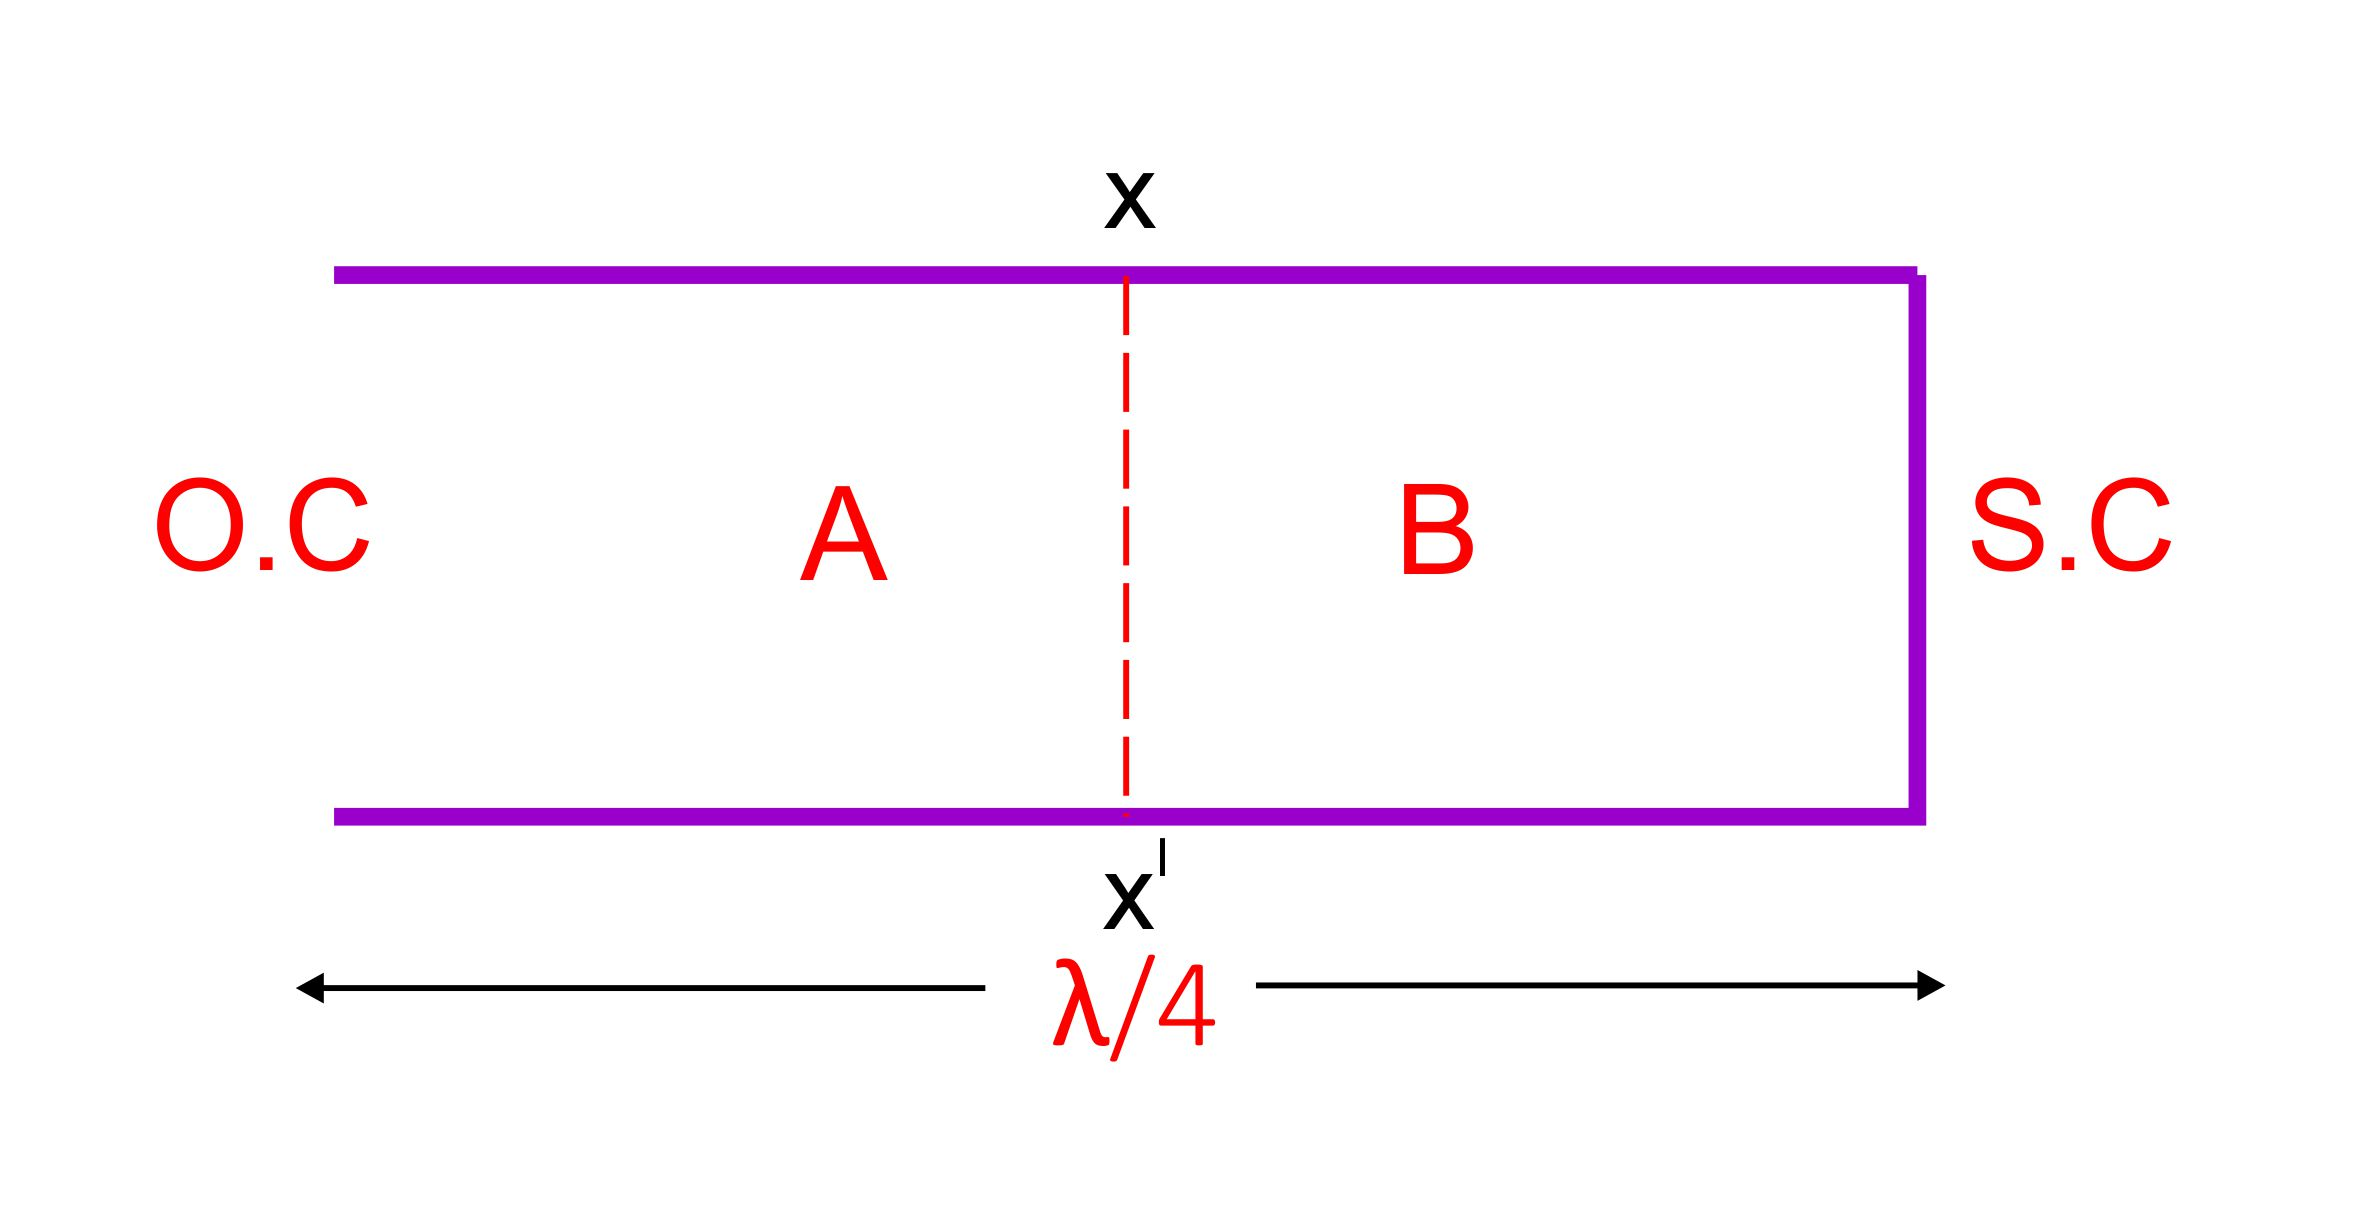
\includegraphics[width=1\linewidth]{./graphics/fig5}
\caption{Short circuit transmission line with section xx'}
\end{figure}

Considering a small section of transmission line shorted at the end shown in figure 11.5. Let's say  by some  means,  voltage  is induced along the section of the  transmission line not from open circuit  or short circuit  end  but between  these  two  points. (let's say at the middle location shown  with  the dotted lines). At any time, it would appear that the two sections (A and B) of transmission lines are connected in parallel. Standing wave signal get setup and induced in the transmission line. This voltage does not see any impedance but the characteristic impedance of the transmission line. So the voltage  at the middle  point XX' sends two traveling waves along the transmission line as if the  energy is supplied to the characteristic impedance of the two sections of the transmission line. The waves are shown  as going in direction M and N respectively. N waves  sees a short circuit and M waves  sees  an open circuit. N sees a reflection  coefficient  of -1. Hence, at short circuit point, the wave is reflected completely as shown  by the arrow. With a reflection coefficient of -1, the amplitude is unity but the phase is 180 degrees. Hence, the wave  traveling toward N after reflection undergoes a phase change of $\pi$ and travels all the way to the open circuit  side as shown by the arrow. At the open circuit point, the reflection coefficient = 1.

$ \Gamma_{L} = \frac{Z_{L} - Z_{o}}{Z_{L} + Z_{o}} =  \frac{1 - \frac{Z_{o}}{Z_{L}}}{1 + \frac{Z_{o}}{Z_{L}}}$\\

$ Z_{L} = \infty $ At open circuit.\\
  
$ \Gamma_{L} =  \frac{1 - \frac{Z_{o}}\infty}{1 + \frac{Z_{o}}\infty} = \frac{1 - 0}{1 + 0} = 1$
   
Hence for open circuit $\Gamma_{L} = 1 $.

And N wave reverses with $\pi$ phase change, it gets to open circuit with a reflection coefficient of  1, turn around and start moving  toward point XX'. Hence at XX' N traveled  a total distance of $ \frac{\lambda}{2} (\frac{\lambda}{8} + \frac{\lambda}{4} + \frac{\lambda}{8})$ and has  gone through a phase change of $2\pi$.

A distance traveled $\frac{\lambda}{4}$ corresponds to a phase change  of $\pi$ due to negative reflection coefficient, it means N has undergone a phase change of $\pi$  (due to $\frac{\lambda }{4}$ distance  traveled) + $\pi$ (due to negative  reflection  coefficient  at short circuit) = $2\pi$ total phase change.

Hence  the  wave induced at XX' is same as the  wave N which has been taken through  a phase change  of $2\pi$. This is some kind of positive feedback because  the induced  voltage  will add to the  reflected  voltage N, increase in amplitude  and the re-traveling process  starts all over. That means  the voltage essentially  starts growing  in  the transmission line. Exactly the same  thing  happen to  wave M. It is reflected  at open circuit point, travels $\frac{\lambda}{4}$ to short circuit  point  reflected with a phase of $\pi$  and travels  towards XX'. At the end has traveled $\frac{\lambda }{2}$  distance  with total phase change of $2\pi$ also. add to the induced  voltage  at XX'. At the end the wave has traveled $\frac{\lambda}{2}$ distance with total phase of $2\pi$ also. Add to the induced voltage at XX'. Then everything  grows as it goes around one more time.  Hence the standing wave of the setup will grow.  Hence a small  voltage is induced at XX'.   
\begin{figure}[h]
\centering
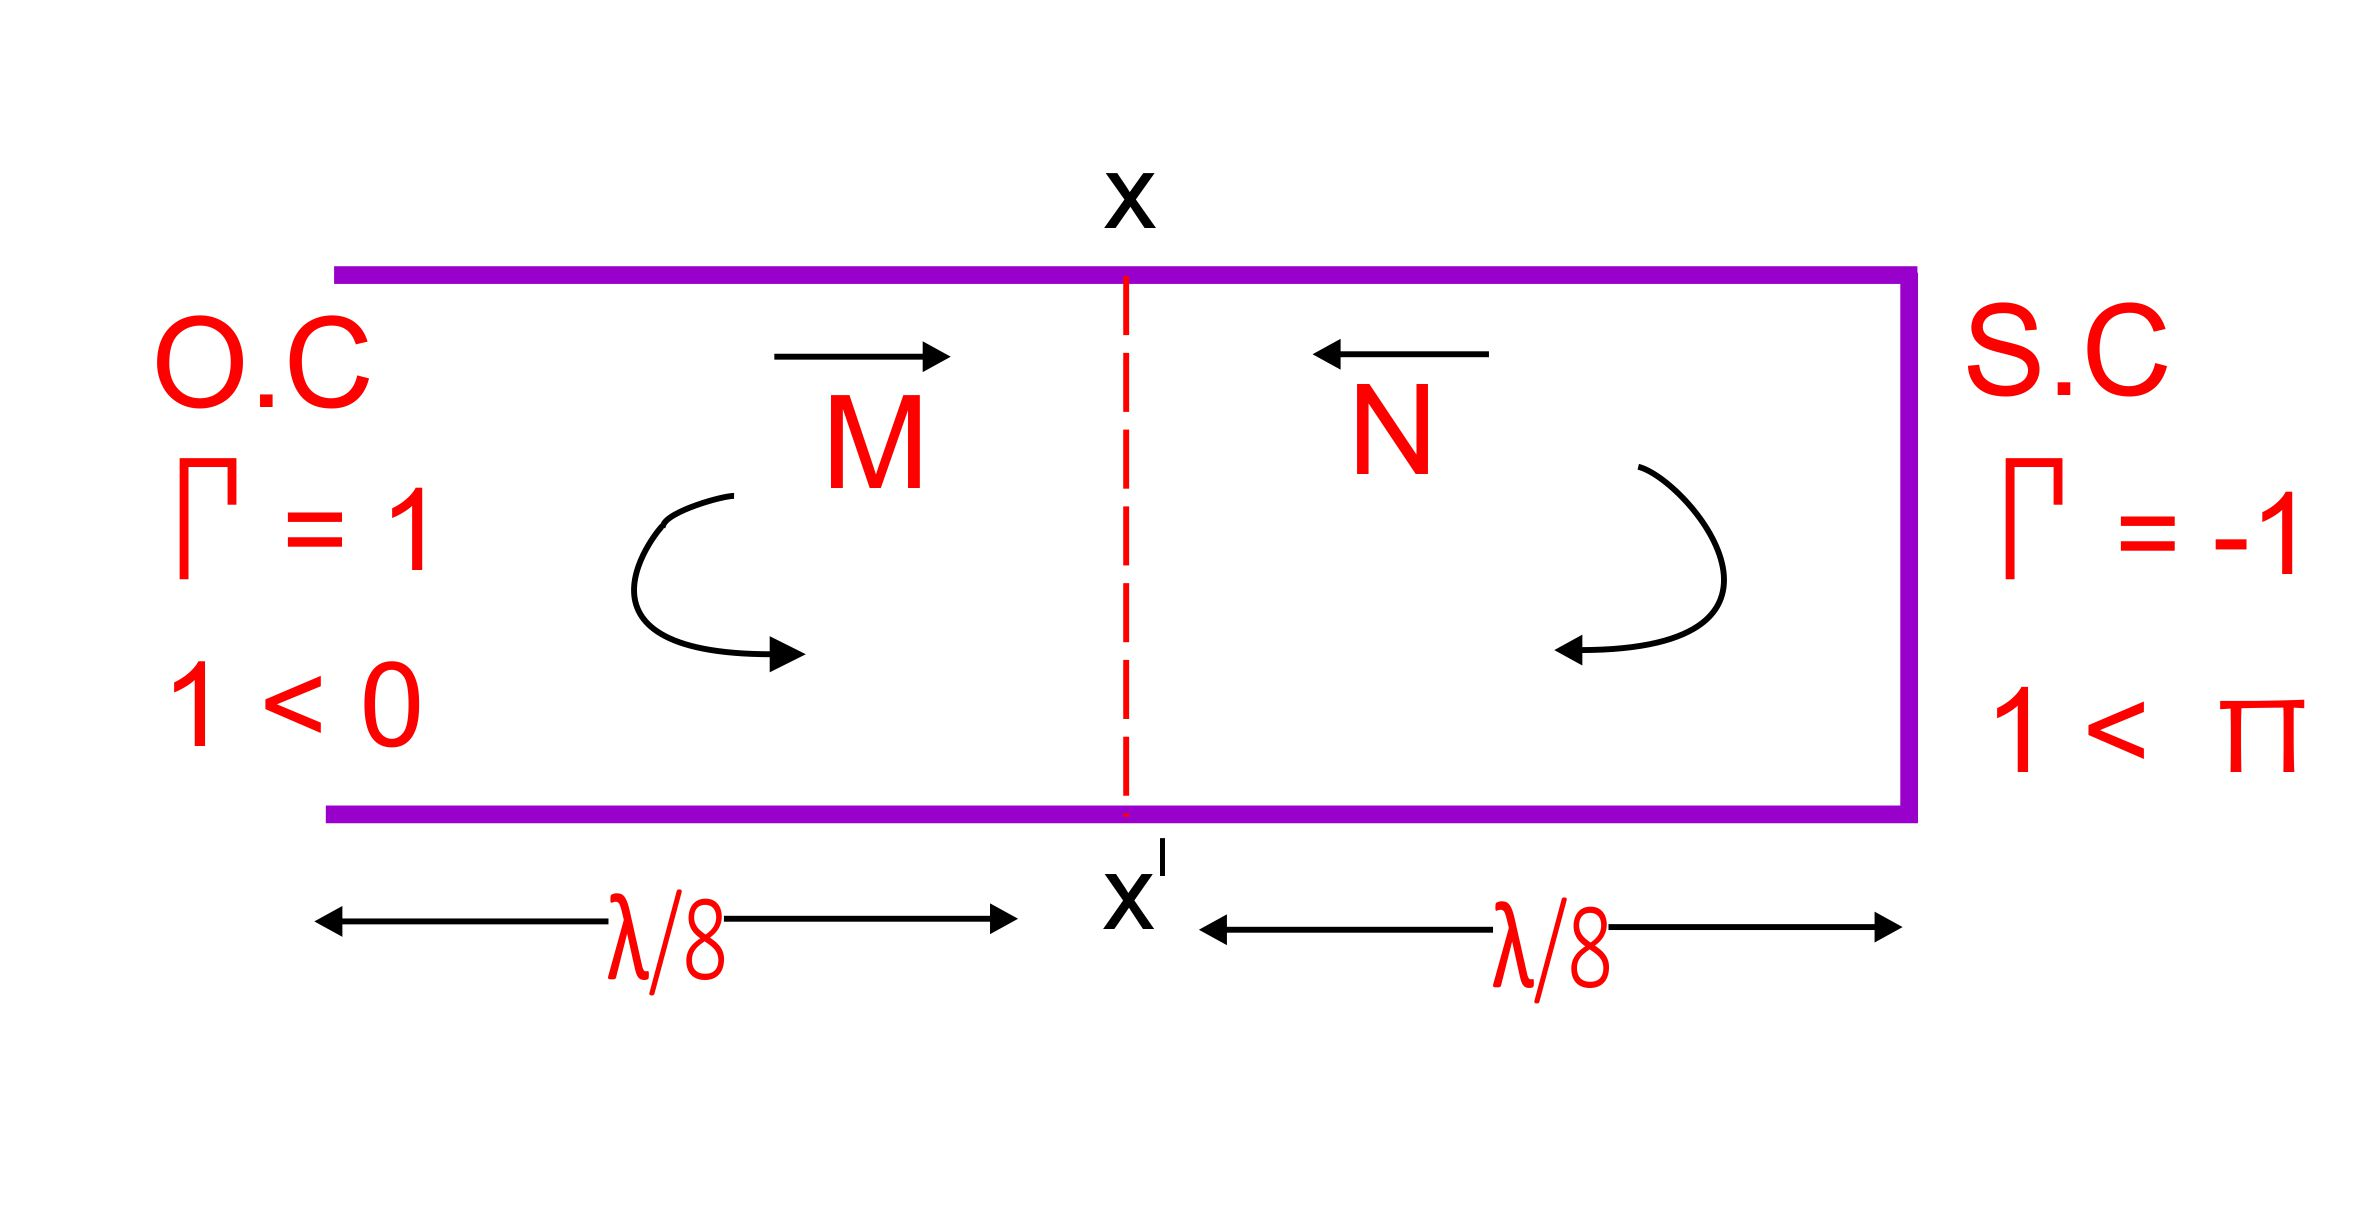
\includegraphics[width=1\linewidth]{./graphics/fig6}
\caption{Short circuit transmission line with with voltage placed at section XX'}
\end{figure}

How far will it grow? With no losses in the transmission line, it will grow up to infinity. The voltage will keep growing to infinite amplitude because there is nothing  controlling this amplitude  on the transmission line. Hence, if even a small voltage is induced on a section  of the transmission line with resonant length, the standing wave in the transmission line is now much larger compared to the induced voltage on the transmission line. This voltage can be used to our advantage in the sense that the voltage  in the transmission line  can be much larger compared to the voltage we originally induced at point XX'.

In order words, this resonance section of a line can be used  as a voltage step up transformer . Hence,  we would  measure  a much  larger  voltage at the open section of the line i.e at open circuit compared  to what we induced at point XX'. With no losses in the line, this voltage  amplitude will grow to infinity. However, that does  not happen because when voltage and current amplitude is increasing in the transmission line, the ohmic losses is increasing. When the losses in  the line due to resistance and conductance (R and G) becomes equal to the  energy source, at that point there is energy balance and the growth of the standing wave in the section of the transmission line stops.

In practice, when the losses are small, one may generate a very large  voltage and current by a small coupling  source  connected  to a section  of the transmission line. This  is a useful application whenever we want to step up voltage or current at high frequencies. It can be shown that this voltage growth is related to the quality factor of transmission line. The higher the quality factor, the lower the losses in the transmission line and that will give higher voltages on the terminal of the transmission line .

The phenomena used here for voltage step up could be harmful in many cases. Consider a situation where a small energy source get unknowingly coupled to a small section of the transmission line. If the section of transmission line is of resonance length, then the voltage developed on this line will be much larger than the circuit can handle and this can damage the circuit. While doing the design of a high frequency circuit, we should be careful not to couple some sections to transmission line especially if they are of resonance length. Else, we develop a large voltage in that section that the circuit can barely handle .  

The phenomenon of stepping up voltage and current in a resonance length when a signal is coupled to it can be used for stepping up voltage or current.
  
For high frequency circuit, when sections of transmission line are used, we rarely see capacitors and inductors at high frequency since they have been replaced by section of transmission line. What we see instead are active devices like transistors and FETs with reactive component completely realized by sections of transmission line. So most microwave circuits will appear as transmission line  across active devices.   